\documentclass{acmsiggraph}               % final
%\documentclass[review]{acmsiggraph}      % review
%\documentclass[widereview]{acmsiggraph}  % wide-spaced review
%\documentclass[preprint]{acmsiggraph}    % preprint

%% Uncomment one of the four lines above depending on where your paper is
%% in the conference process. ``review'' and ``widereview'' are for review
%% submission, ``preprint'' is for pre-publication, and ``final'' is for
%% the version to be printed.

%% These two line bring in essential packages: ``mathptmx'' for Type 1
%% typefaces, and ``graphicx'' for inclusion of EPS figures.

\usepackage{mathptmx}
\usepackage{graphicx}

%% use this for zero \parindent and non-zero \parskip, intelligently.

%\usepackage{parskip}
\usepackage{subfigure}
\usepackage{smrdefaults}

%% If you are submitting a paper to the annual conference, please replace
%% the value ``0'' below with your OnlineID. If you are not submitting this
%% paper to the annual conference, you may safely leave it at ``0'' -- it
%% will not be included in the output.

\onlineid{0}

%% need to document this!

\acmformat{print}

%% Paper title.

\title{TAPESTREA: Sound Scene Modeling By Example}

%% Author and Affiliation (single author).

\author{Ananya Misra, Perry R. Cook, and Ge Wang\\Princeton 
University\thanks{e-mail: \{amisra, prc, gewang\}@cs.princeton.edu}}

%% Author and Affiliation (multiple authors).

%%\author{Roy G. Biv\thanks{e-mail: roy.g.biv@aol.com}\\ Starbucks Research %
%%\and Ed Grimley\thanks{e-mail:ed.grimley@aol.com}\\ Grimley Widgets, Inc. %
%%\and Martha Stewart\thanks{e-mail:martha.stewart@marthastewart.com}\\ Martha Stewart Enterprises \\ Microsoft Research}

%% Keywords that describe your work.

%\keywords{sound scene, synthesis, sinusoidal modeling, wavelet}
% should sound texture be a keyword?

%%%%%% START OF THE PAPER %%%%%%

\begin{document}

\teaser{
\center
\includegraphics[width=6.0in]{teaser3.jpg}
% \subfigure[original]{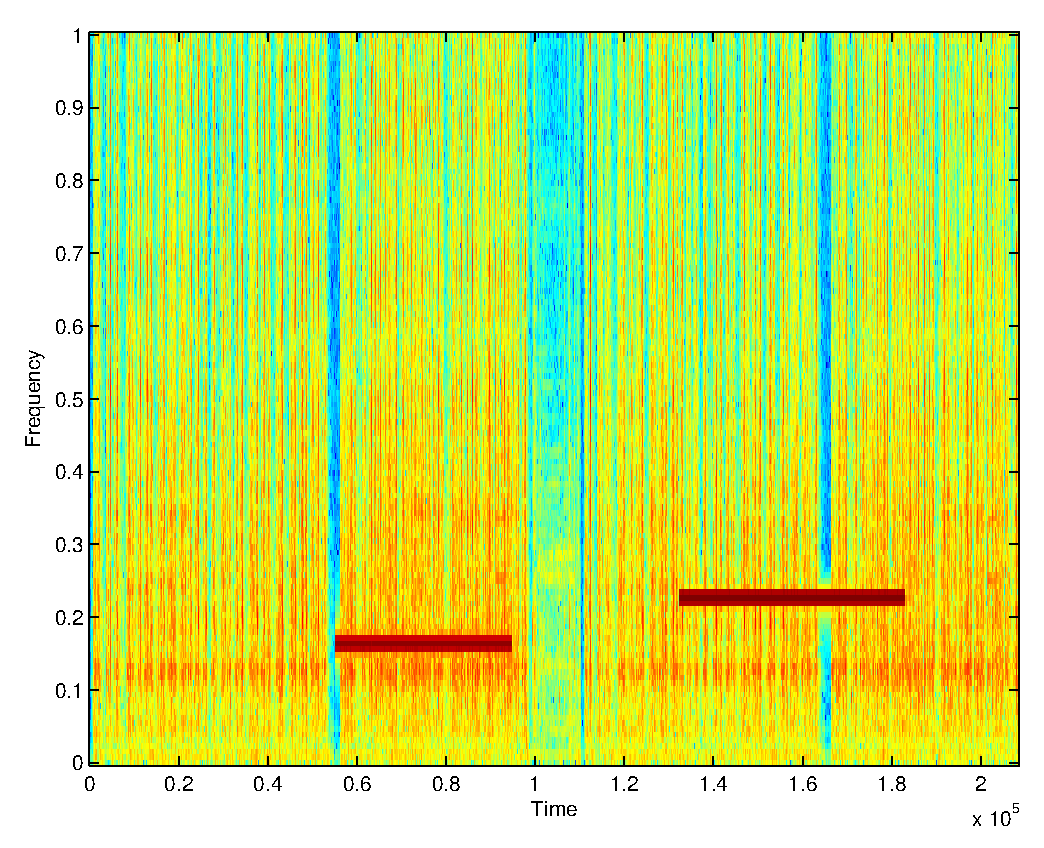
\includegraphics[width=.24\textwidth]{story1.eps}}
% \subfigure[foreground]{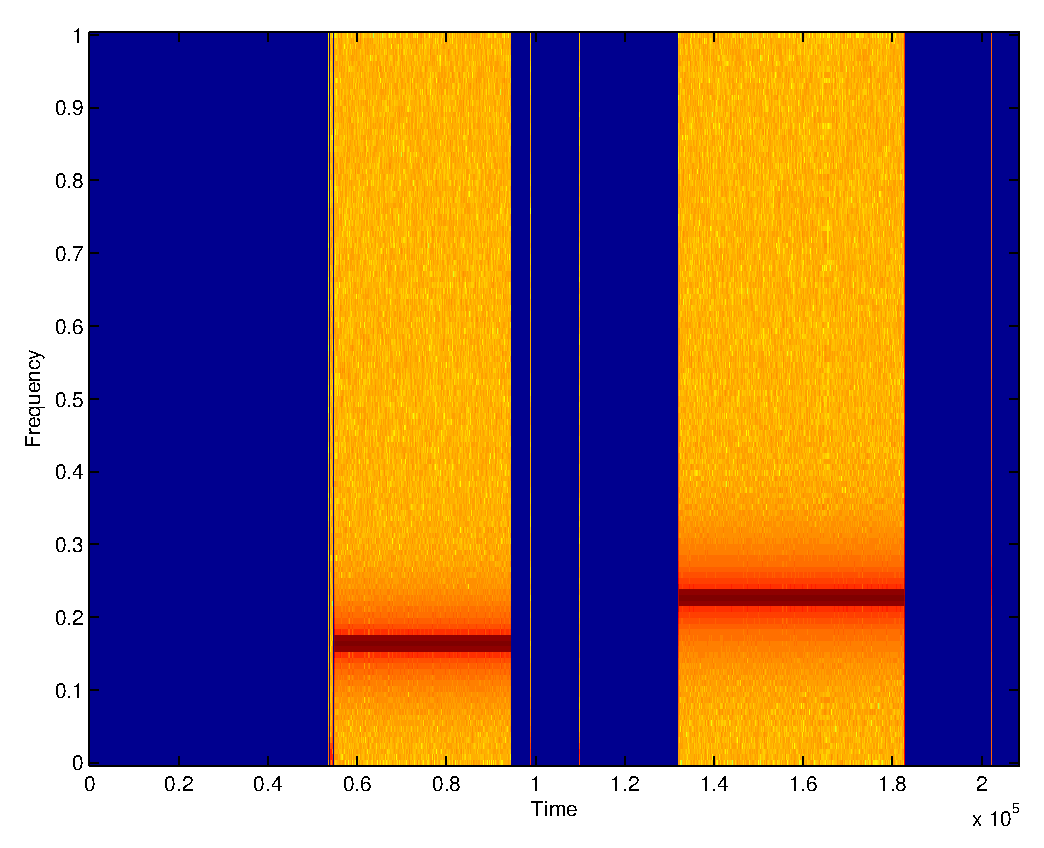
\includegraphics[width=.24\textwidth]{story2.eps}}
% \subfigure[background]{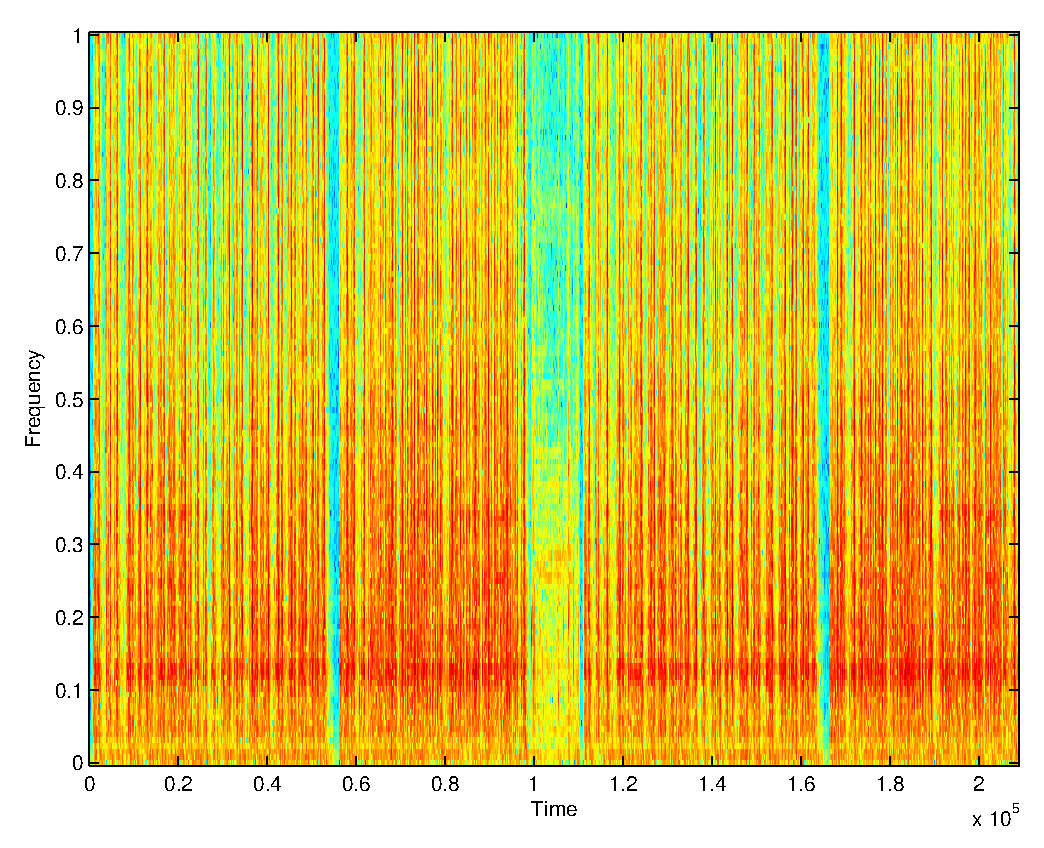
\includegraphics[width=.24\textwidth]{story3_fake.eps}}
% \subfigure[synthesized]{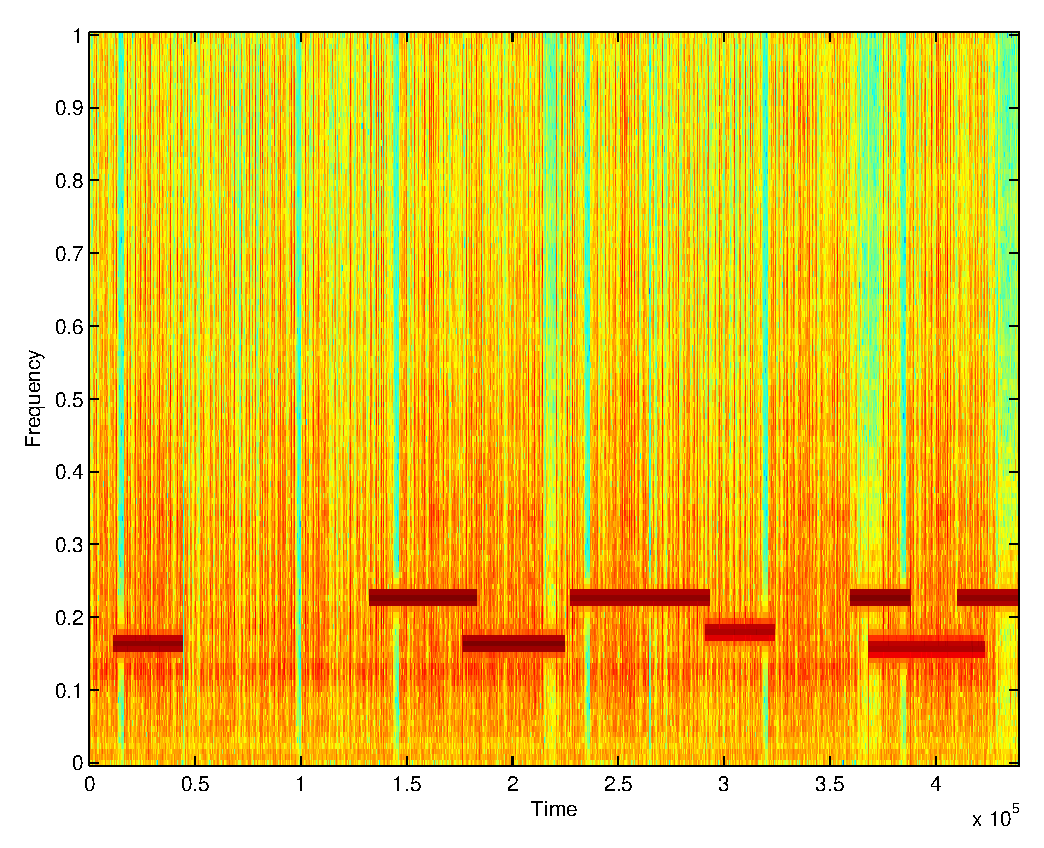
\includegraphics[width=.24\textwidth]{story4_fake.eps}}
  \caption{ A sound scene composed of background and foreground elements
from several existing scenes }
  \label{fig:teaser}
}

% The ``\maketitle'' command must be the first command after the
% ``\begin{document}'' command. It prepares and prints the title block.

\maketitle

\section{Introduction}

We present a new paradigm and framework for creating high-quality ``sound
scenes'' from a set of recordings. A sound scene is a
combination of background and foreground sounds that together evoke the
sense of being in a specific environment. The ability to craft and control
sound scenes is important in entertainment (movies, TV, games), 
virtual/augmented reality, art projects (live performances, installations) 
and other multimedia applications.

Existing audio production tools require ``untainted'' versions of 
sound components and frequently involve tedious event-by-event editing.
No system, to our knowledge, provides an arena for truly flexible
``sound scene modeling by example,'' where a sound scene can be composed
from selected, extracted, and separated components of different existing 
scenes. We introduce a parametric, unified framework of analysis, 
transformation and synthesis techniques that allow users to interactively 
select components from existing sounds, transform these independently, 
and controllably recombine them to create new sound scenes in real-time. 
We call this system TAPESTREA: Techniques and Paradigms for Expressive 
Synthesis, Transformation and Rendering of Environmental Audio.

\section{Techniques and Paradigms}

Our approach follows from the notion that sound scenes are composed of
discrete events as well as background sound, and these are best modeled 
separately.  A sound scene is separated into the following components:
(1) {\it deterministic events}: composed of sinusoids, often
perceived as pitched events, such as a bird chirp or a voiced vowel,
(2) {\it transient events}: brief non-sinusoidal events, such as
footsteps, 
(3) {\it stochastic background}: the ``din'' remaining after the
removal of foreground events, such as wind or street noise.

Our parametric analysis interfaces let a user extract selected instances 
of any component type from a given sound scene, and save them as {\it
templates} for future use in corresponding transformation and synthesis
interfaces.

Our system benefits from employing separate analysis and synthesis
algorithms for each component type. We apply spectral modeling
~\cite{Serra89} to extract deterministic events, and resynthesize 
them with optionally massive time and frequency transformations.
Transient events are isolated by locating sudden increases in time-domain
signal energy, and are replayed directly or with time-frequency
transformations.  Both event types are removed from the original sound to
obtain the background. Deterministic events are removed by
sinusoidal track detection, while removed transient events are ``filled in'' or replaced 
using wavelet tree learning ~\cite{Dubnov02} of nearby 
transient-free segments.  An improved wavelet tree learning 
technique also synthesizes continuous, non-repeating stochastic 
background sound, similar to the extracted background template.

A user, having extracted templates, can parametrically resynthesize them
with specific individual real-time transformations. The system also offers
structures for explicitly placing events in time at many granularities,
and for synthesizing repeating events at controllable periodicity,
density, and random-transformation ranges, useful for generating crowd
sounds from a single template. Together, these enable the production of a
wide range of sound scenes, of any desired length, from a static and 
limited set of recordings.

\section{Contributions}

Our main contributions include: (1) techniques and paradigms 
for interactive template selection and extraction, (2) techniques for 
parametrically transforming components independently, (3) a framework for 
flexible resynthesis to create novel sound scenes, (4) interfaces 
to facilitate each task in the analysis and synthesis pipeline. 
Most significant are the new  
approach, system, and interface for modeling sound scenes by example.

% These include interfaces to facilitate
% each phase in the process, extensions to the existing algorithms used, and
% a cohesive framework for selective template extraction, independent
% transformations, and flexible resynthesis.

\bibliographystyle{acmsiggraph}
\nocite{*}
\bibliography{sketch}
\end{document}
